\documentclass{article}
\usepackage{graphicx} % Required for inserting images
\usepackage[margin=1in]{geometry}
\usepackage{amsmath}
\usepackage{amsfonts}
\usepackage{listings} % to write code 
\usepackage{mathabx} % \boxslash
\usepackage{float}


\title{Tensor Factorisation for Group Detection}
\author{ Ange Kokotakis, Romain Ramez \\ \small directed by Rodrigo Cabral Farias}
\date{December 2023}

\begin{document}

\maketitle

\begin{abstract}
    The aim of this project is to detect groups of people with a given dataset of interactions in a community.
    For this purpose we will represent the dataset as a tensor and use non-negative tensor factorization to approximate
    it as a product of different matrix from which we can get information about groups in this community.
\end{abstract}

\section{Introduction}

Group detection can be very important in different cases. These identified groups serve as fundamental pillars for predictive modeling, providing insights into future behaviors, trends, and interactions.
Indeed, from simple contacts, being able to detect a group and its dynamics is not so simple, certain groups can mix and others can remain isolated. We must be able to separate a simple contact between two people from a group relationship.
For this, we will use two models: MU and HALS.
We will compare them and see which is the most effective and durable.

\section{Model}

In this project, we use datasets similar to Figure \ref{dataset} in which each line represents an interaction between
two individuals: $id1$ and $id2$ at a certain $time$.

\begin{figure}[H]
    \centering
    \includegraphics[width=0.3\textwidth]{images/tableau_données.png}
    \caption{dataset}
    \label{dataset}
\end{figure}

From this dataset we create matrices $\mathbf{X} \in \{0, 1\}^{I \times I}$ which represent interactions between people during a certain
interval of time where $I$ is equal to the number of people in the community and each coefficient is equal to :

\[
    \mathbf{X}_{i,j} = 
    \begin{cases}
        1 & \text{if there is an interaction between person $i$ and $j$ during a given interval of time} \\
        0 & \text{otherwise}
    \end{cases}
\]

And then we stack these matrices with different interval $t_k$ of time to create our tensor $\mathbf{Y} \in \{0, 1\}^{I \times I \times K}$
where K is the number of intervals of time. Finally the tensor containing the dataset has its coefficients equal to :

\[
    \mathbf{Y}_{i,j,k} = 
    \begin{cases}
        1 & \text{if there is an interaction between person $i$ and $j$ at interval of time $t_k$} \\
        0 & \text{otherwise}
    \end{cases}
\]

In order to approximate this tensor we create 3 matrices :
\[
    \mathbf{U} \in \mathbb{R}_+^{I \times R}, \,
    \mathbf{V} \in \mathbb{R}_+^{I \times R}, \,
    \mathbf{W} \in \mathbb{R}_+^{K \times R}
\]

where :
\begin{itemize}
    \item[]
    \begin{itemize}
        \item $I$ is the number of individuals in the community,
        \item $K$ is the number of interval of time,
        \item $R$ is the number of groups in the community (we choose one randomly at first we will see later how to choose it correctly).
    \end{itemize}
\end{itemize}

The $U$ and $V$ matrices represent the membership level of a person to a certain group
and $W$ represents in which interval of time a group has been active.

% \[
%     L(U, V, W)=\|Y-[U, V, W]\|_{F}^2 +\lambda \|U-V\|_{F}^2
% \]

%\section{Multiplication Update Algorithm (MU)}

% \begin{lstlisting}[language=Python]
    % code
% \end{lstlisting}

We define $\mathbf{S} \in \mathbb{R}_+^{I \times I \times K}$ as :

\[
    \mathbf{S}_{i,j,k} = \sum_{r = 1}^R \mathbf{U}_{i,r}\mathbf{V}_{j,r}\mathbf{W}_{k, r}
\]

The result of the product $\mathbf{U}_{i,r}\mathbf{V}_{j,r}\mathbf{W}_{k, r}$ is called the outer product noted $\mathbf{U}_r \circ \mathbf{V}_r \circ \mathbf{W}_r$ which can be seen as :

\begin{figure}[H]
    \centering
    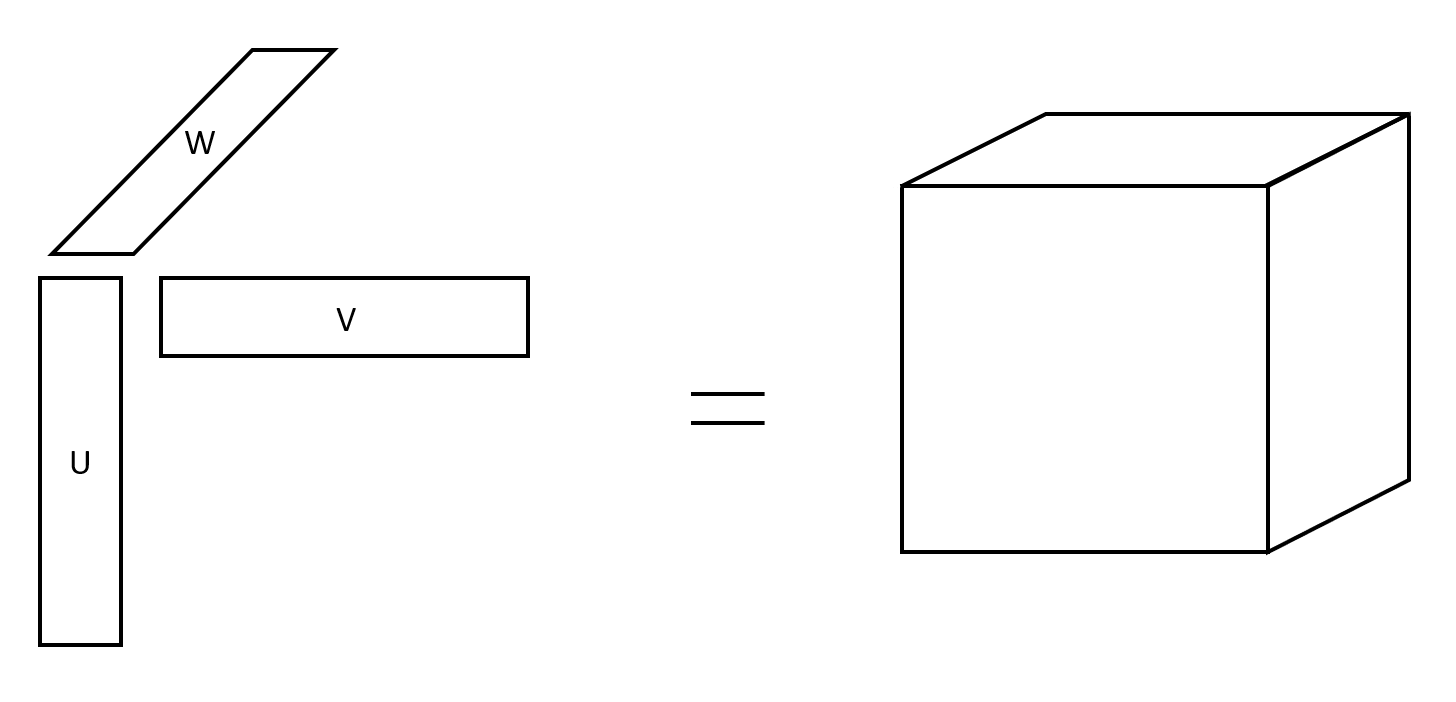
\includegraphics[width=0.5\textwidth]{images/outer_product.png}
\end{figure}


Finally S is define as : 
\[
    \mathbf{S} = \sum_{r = 1}^R \mathbf{U}_r \circ \mathbf{V}_r \circ \mathbf{W}_r
\]

In order to approximate Y with S we define a cost fonction $L(\mathbf{U}, \mathbf{V}, \mathbf{W})=\|\mathbf{Y}-\mathbf{S}\|_{F}^2$ where $\|.\|_F$ represents the Frobenius norm,
moreover because U and V are representing the same thing we want these matrices to be similar so we add to L another term $\lambda\|\mathbf{U}-\mathbf{V}\|_{F}^2$.
 Finally $L$ is defined by :

\[
    L(\mathbf{U}, \mathbf{V}, \mathbf{W})=\|\mathbf{Y}-\mathbf{S}\|_{F}^2 +\lambda \|\mathbf{U}-\mathbf{V}\|_{F}^2, \lambda \in \mathbb{R}_+
\]

$L$ can be rewritten by using unfolded forms of $\mathbf{Y}$ i.e. by transforming it in a matrix with all the layers of $\mathbf{Y}$
arranged in different ways, and by using Khatri-Rao product $\odot$ :

\begin{align*}
L(\mathbf{U}, \mathbf{V}, \mathbf{W}) &= \|\mathbf{Y}^{(1)}-\mathbf{U}(\mathbf{W}\odot \mathbf{V})^{T}\|_{F}^2 +\lambda \|\mathbf{U}-\mathbf{V}\|_{F}^2 \\
                &= \|\mathbf{Y}^{(2)}-\mathbf{V}(\mathbf{W}\odot \mathbf{U})^{T}\|_{F}^2 +\lambda \|\mathbf{U}-\mathbf{V}\|_{F}^2\\
                &= \|\mathbf{Y}^{(3)}-\mathbf{W}(\mathbf{V}\odot \mathbf{U})^{T}\|_{F}^2 +\lambda \|\mathbf{U}-\mathbf{V}\|_{F}^2
\end{align*}

To minimize this function we will use two
different method : the multiplicative update algorithm (MU) and the hierarchical alternating least square (HALS) and these forms of
$L$ will be very useful.

\section{Multiplicative Update}
The principle of this algorithm is to alternatively minimize $L$ with respect to each of its components by
using a version of gradient algorithm.

At each iteration we calculate :

\[\nabla L = \begin{bmatrix}
                \nabla_{\mathbf{U}} L\\
                \nabla_{\mathbf{V}} L \\
                \nabla_{\mathbf{W}} L 
            \end{bmatrix} = \begin{bmatrix}
                                [\nabla_{\mathbf{U}} L]^{+}-[\nabla_{\mathbf{U}} L]^{-}\\
                                [\nabla_{\mathbf{V}} L]^{+}-[\nabla_{\mathbf{V}} L]^{-} \\
                                [\nabla_{\mathbf{W}} L]^{+}-[\nabla_{\mathbf{W}} L]^{-} 
                            \end{bmatrix}
\]

Where all the $[.]^{+}, [.]^{-}$ are positive

Then we update $\mathbf{U}, \mathbf{V}$ and $\mathbf{W}$ :
\begin{align*}
    &\mathbf{U}_{k} = \mathbf{U}_{k-1}\boxdot ([\nabla_{\mathbf{U}} L]^{+}\boxslash[\nabla_{\mathbf{U}} L]^{-}) \\
    &\mathbf{V}_{k} = \mathbf{V}_{k-1}\boxdot ([\nabla_{\mathbf{V}} L]^{+}\boxslash[\nabla_{\mathbf{V}} L]^{-}) \\
    &\mathbf{W}_{k} = \mathbf{W}_{k-1}\boxdot ([\nabla_{\mathbf{W}} L]^{+}\boxslash[\nabla_{\mathbf{W}} L]^{-})
\end{align*}
Where $\boxdot$ and $\boxslash$ are the Hadamard product and division respectively. To avoid division by zero, we replace all the zero coefficient in $[.]^{+}$ by an epsilon strictly positive.




\section{Hierarchical Alternating Least Square}
This algorithm minimize $L$ with respect to one column of $\mathbf{U}$, $\mathbf{V}$ or $\mathbf{W}$ at a time, all the other column are fixed to their previous approximation
for instance with the column $\mathbf{U}_{r'}$ :

\begin{align*}
      &\,\, L = \|\mathbf{Y}-\mathbf{S}\|_{F}^2 +\lambda \|\mathbf{U}-\mathbf{V}\|_{F}^2 \\
      &= \sum_{ijk}(\mathbf{Y}_{ijk}-\sum_{r \ne r'}(\mathbf{U}_{ir}\mathbf{V}_{jr}\mathbf{W}_{kr})-\mathbf{U}_{ir'}\mathbf{V}_{jr'}\mathbf{W}_{kr'})^{2}+\lambda\sum_{i}\sum_{r \ne r'}(\mathbf{U}_{ir}-\mathbf{V}_{ir})^{2}+\lambda\sum_{i}(\mathbf{U}_{ir'}-\mathbf{V}_{ir'})^{2}\\
      &= \sum_i \mathbf{U}_{ir'}^2(\lambda I + \sum_{jk}(\mathbf{W}_{kr'}\mathbf{V}_{kr'})^2) - 2 \mathbf{U}_{ir'}(\lambda \mathbf{V}_{ir'} + \sum_{jk}\mathbf{W}_{kr'}\mathbf{V}_{kr'}(\mathbf{Y}_{ijk}-\sum_{r \ne r'}(\mathbf{U}_{ir}\mathbf{V}_{jr}\mathbf{W}_{kr}))) + C , \text{C independent of $\mathbf{U}_{ir'}$ }\\
      &\text{So $L$ is minimum with respect to $\mathbf{U}_{ir'}$ if } \mathbf{U}_{ir'} = \frac{\lambda \mathbf{V}_{ir'} + \sum_{jk}\mathbf{W}_{kr'}\mathbf{V}_{kr'}(\mathbf{Y}_{ijk}-\sum_{r \ne r'}(\mathbf{U}_{ir}\mathbf{V}_{jr}\mathbf{W}_{kr}))}{\lambda I + \sum_{jkr'}(\mathbf{W}_{kr'}\mathbf{V}_{kr'})^2}
\end{align*}

We can generalize this result to an entire column : $\mathbf{U}_{:,r'} = \frac{\lambda \mathbf{V}_{:,r'} + \sum_{jk}\mathbf{W}_{kr'}\mathbf{V}_{kr'}(\mathbf{Y}_{:,jk}-\sum_{r \ne r'}(\mathbf{U}_{:,r}\mathbf{V}_{jr}\mathbf{W}_{kr}))}{\lambda I + \sum_{jkr'}(\mathbf{W}_{kr'}\mathbf{V}_{kr'})^2}$,
we can find the two other update by symetry for $\mathbf{V}$ and by doing the same calcul for $\mathbf{W}$.\\

At each iteration we update $\mathbf{U}_{r'}$, $\mathbf{V}_{r'}$, $\mathbf{W}_{r'}$,  then we increment $r'$ until we reach our convergence criterion or our maximum number of iteration.

\section{Comparison of MU and HALS convergence}

We note that MU converge faster than HALS.

\begin{figure}[H]
    \centering
    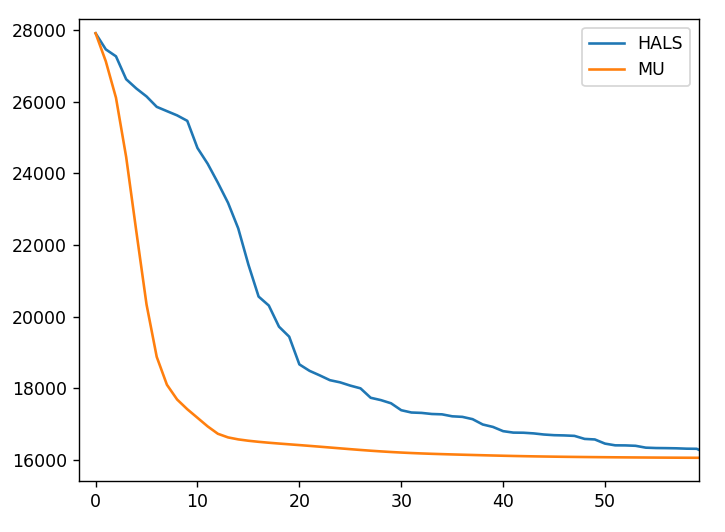
\includegraphics[width=0.5\textwidth]{images/comparison_HALS_MU.png}
    \caption{comparison between MU and HALS convergence}
\end{figure}

\section{Interpretation of our results}

In this section we use a database composed of interaction between students and teachers in a school during 2 days, this databse furnished
metadata which indicate in which class students are. We represent it as the scheme below where two people in the same class have the same color, teachers ar in black,
the distance between two individuals is randomly chosen and have no meaning in this representation :

\begin{figure}[H]
    \centering
    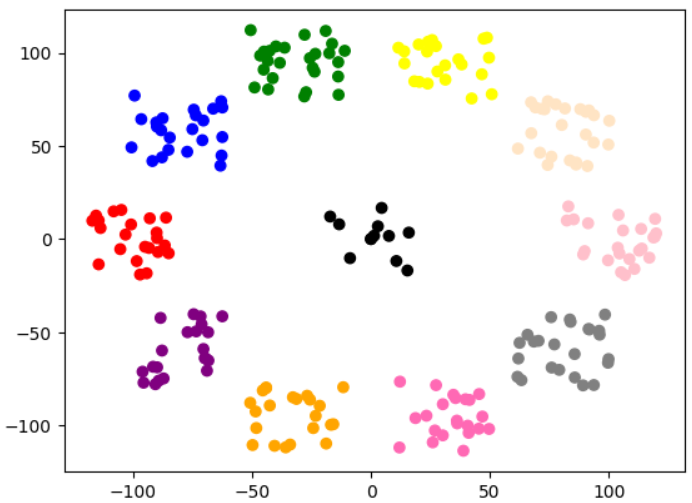
\includegraphics[width=0.5\textwidth]{images/original_class.png}
    \caption{original classes}
\end{figure}

\subsection{A first approximation}
Using $\mathbf{U}$ (or $\mathbf{V}$) we create the same representation by choosing the maximum in each line of U to determine the group of a person in the school,
we naively chose R = 11 because we can see 11 groups on the scheme above, it give us this in the best case:

\begin{figure}[H]
    \centering
    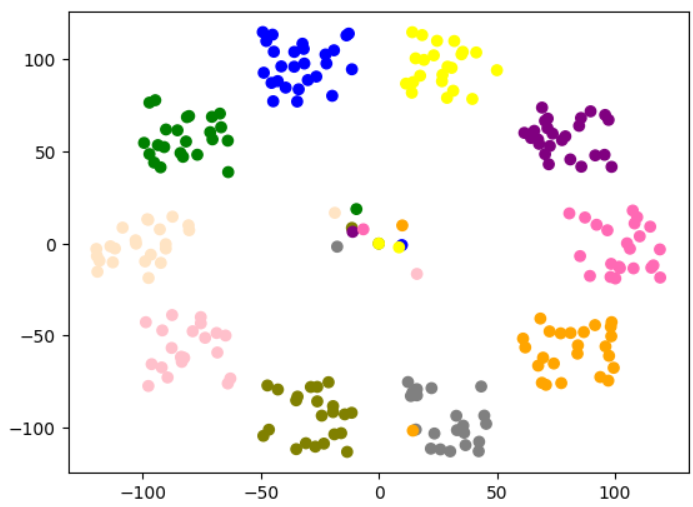
\includegraphics[width=0.5\textwidth]{images/naive_approach_r=11_t=18000.png}
    \caption{estimation with R = 11, timestep = 18000$s$}
\end{figure}

As we can see, the group of teachers is not well approximate. It can be easily explained by the fact that they have way more 
interactions with students over a day than with other professor. By checking the original database, interactions between two teachers 
represents less than 7.5\% of the total numbers of interactions between a professor and someone else. 
So teachers will finally be part of classes group and cant be detected by this model.\\

\subsection{Impact of initial conditions}
By doing this first factorization we noticed that, with these parameters, the approximation is not every time the same, 
no matter the number of iteration we do. The model is sensitive to the initial $\mathbf{U}$, $\mathbf{V}$ and $\mathbf{W}$ that we
choose randomly at the intialisation. We have mainly 3 cases :

\begin{figure}[H]
    \centering
    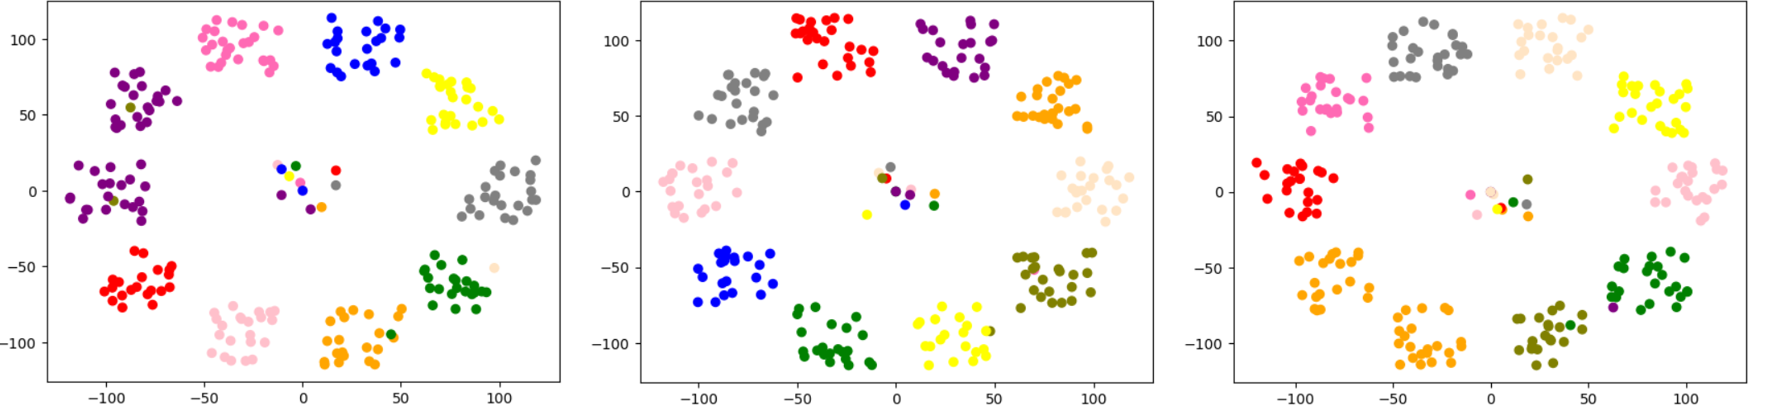
\includegraphics[width=1\textwidth]{images/3cases_of_convergence.png}
    \caption{3 differents estimations with R = 11, timestep = 18000$s$}
\end{figure}

In these 3 cases the value of L are nearly the same, we deduce from these estimations that the function L has different local minimum, so the model can converge 
towards different solutions depending of the initial $\mathbf{U}$, $\mathbf{V}$ and $\mathbf{W}$.

\subsection{impact of R}

We have seen above that we can realistically define 10 groups in this school, but what happened if we choose to reduce or increase this number ?
Lets start wit $R = 5$ :\\

\begin{figure}[H]
    \centering
    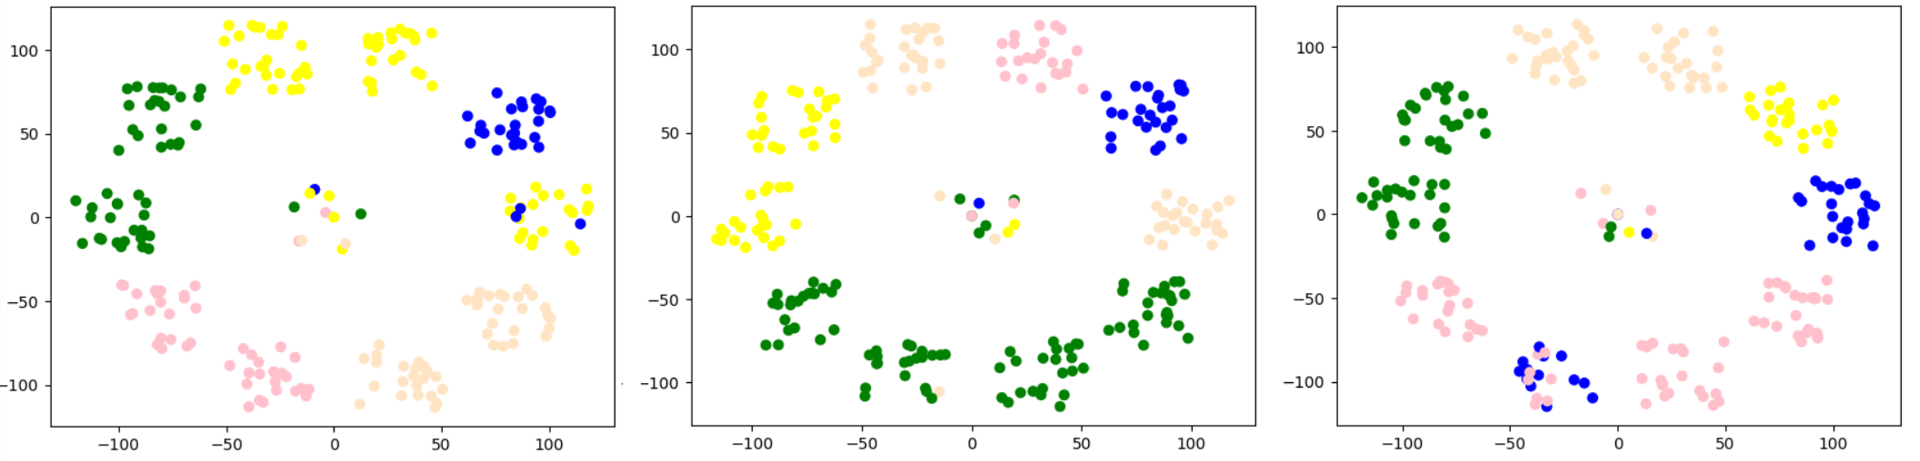
\includegraphics[width=1\textwidth]{images/R=5_t=18000.png}
    \caption{estimations with R = 5, timestep = 18000$s$}
\end{figure}

With $R = 5$, we try to put a larger number of group in only 5 groups. We can see that the model try to regroup some of the original groups
together. That's why we have lots of originals groups in the same color. We still have well separated groups it shows that
the model is still efficient. We can see, globally, that all the people from each original group are together in one of the five biger groups.\\

Now, lets see with $R = 15$ :

\begin{figure}[H]
    \centering
    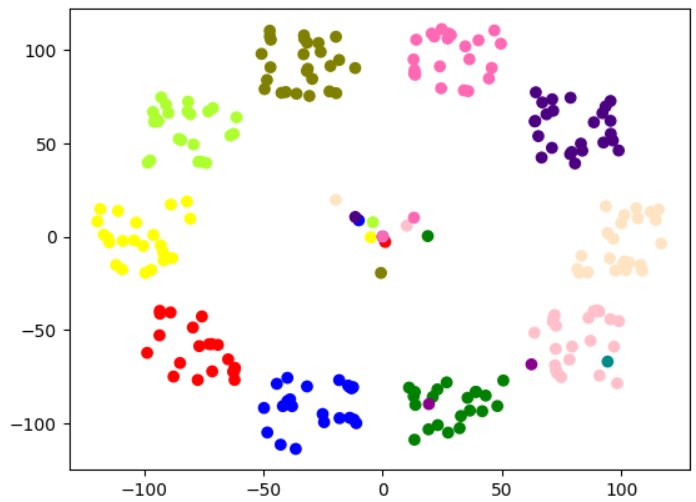
\includegraphics[width=0.5\textwidth]{images/R=15_t=18000.png}
    \caption{estimations with R = 15, timestep = 18000$s$}
\end{figure}

With $R = 15$, we have nearly always the same result, which is a good thing : it reduces the uncertainty caused by the initial conditions.
Moreover we can see that despite the fact that $R = 15$, the model only created 12 groups and there is a group with only 1 member : the cyan one, and another with only
2 members: the light purple one. So having a $R$ slightly above the real one is actually useful to have a better approximation.

\subsection{Impact of timestep}
We tested a lot of different timestep with different $R$ and their is no real impact on $\mathbf{U}$ and $\mathbf{V}$,
the only thing we can say is that the more the timestep is little the more $\mathbf{W}$ will be precise.

\subsection{Analysis of groups activity over time}

Using W we can interpret when groups has been active over time. Lets start with a timestep equals to 3600 which is equivalent to one hour,
W will be represented as a scheme where coefficient are colors, the more the color is close to purple the more coefficient is close to 0, the more
the color is close to yellow the more coefficient is close to 1.

\begin{figure}[H]
    \centering
    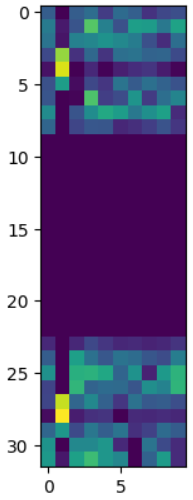
\includegraphics[width=0.2\textwidth]{images/W_R=10_t=3600.png}
    \caption{W with R = 10, timestep = 3600$s$}
\end{figure}

The experiment has been done on 2 days, we can easily see night because there is no activities on a long period.Then we can identify
2 types of groups : friends groups and classes groups, indeed most of the groups have less interactions during the launch break (line 4 and 28)
and have many interactions during class, these groups are classes groups. And the column 2 correspond to a group of friends who have
no interactions during class and a lot of interactions at launch.

\section{Bibliographie}
\begin{enumerate}
    \item \textbf{\textit{Fast Local Algorithms for Large Scale Nonnegative Matrix and Tensor Factorizations}} \\
    \textit{Researchgate}
    
    \item \textbf{\textit{Detecting the Community Structure and Activity Patterns of Temporal Networks: A Non-Negative Tensor Factorization Approach}} \\
    Laetitia Gauvin, André Panisson, Ciro Cattuto
    
    \item \textbf{\textit{Contact Patterns among High School Students}} \\
    Julie Fournet, Alain Barrat
    
    \item \textbf{\textit{The Why and How of Nonnegative Matrix Factorization}} \\
    Nicolas Gillis
    
    \item \textbf{\textit{Learning the Parts of Objects by Non-Negative Matrix Factorization}} \\
    Daniel D. Lee, H. Sébastien Seung
    
    \item \textbf{\textit{Tensor Decompositions and Applications}} \\
    Tamara G. Kolda, Brett W. Bader
    
    \item \textbf{\textit{High-Resolution Measurements of Face-to-Face Contact Patterns in a Primary School}} \\
    Juliette Stehlé, Nicolas Voirin, Alain Barrat, Ciro Cattuto, \\
    Lorenzo Isella, Jean-François Pinton, Marco Quaggiotto, \\
    Wouter Van den Broeck, Corinne Régis, Bruno Lina, \\
    Philippi Vanhems
    
    \item \textbf{\textit{Advanced Data Mining}} \\
    Rodrigo Cabral
    
    \item \textbf{\textit{The Matrix Cookbook}} \\
    Kaare Brandt Petersen, Michael Syskind Pedersen
\end{enumerate}

\end{document}
%mettre en gras les matrices en gras voir mathbf